%! TeX root = ../charles/en/thesis.tex
\chapter{Method}
\label{chap:method}

\section{Probing Temporal Ability}
\label{sec:prob}

\XXX{With the current limited writeup, Ondrej cannot comment yet. Some critical remarks: always try hard to complement other people's scores (which you can cite from a paper) with \emph{your own measurement} of their outputs. Typically, these reported and re-measured numbers will differ and it is always important to know them for a reliable comparison with your own scores.}

Table on changing temporal indicators improving performance on STAR
\begin{table}[htpb] 
    \centering 
    \caption{Results of Merlot Reserve on STAR dataset. Differences explained  
        by different sampling techniques I think, or question-statement 
        conversions. I took care to adapt the statements appropriately for verb 
        tense agreement. Also random seed may be different.For val, 43.01 mean 
        is weighted by num in each group.} 
    \label{tab:star} 
    \begin{tabular}{c|ccccc} 
        & Interaction & Sequence & Prediction & Feasibility & Mean \\
        \hline 
        Val & 43.12 & 42.33 & 43.27 & 47.14 & 43.01 (43.97) \\
        Test & 40.51 & 44.76 & 43.85 & 39.48 & 42.15 \\  
        Test Paper (B+audio) & 44.8 & 42.4 & 38.8 & 36.2 & 40.5 
    \end{tabular} 
\end{table} 

Switch before/after: 42.92 vs 42.33 with correct temporal ordering
%TODO: get test results for this as well

Use before/after as MASKed answers: 50.86 (basically random)

\begin{table}[htpb]
    \centering
    \caption{Shuffle frames (randomly)}
    \label{tab:shuf}
    \begin{tabular}{c|cccc|c}
        & Interaction & Sequence & Prediction & Feasibility & Mean \\
        \hline
        Standard & 43.12 & 42.33 & 43.27 & 47.14 & 43.01 (43.97) \\
        Shuffle & 42.08 & 42.58 & 47.28 & 49.2 & 43.28 (45.29) \\
    \end{tabular}
\end{table}

\section{Experiment Setup}
\label{sec:setup}

\subsection{Dataset Creation}
\label{sec:data}

We finetune the Merlot Reserve model on the Charades dataset. For each video,
we create relation pairs based on annotated actions. Each relation is based on
Allen's Interval Algebra~\citep{allen1983interval}, shown in Table
\ref{tab:allen_interval}.

\begin{table}[htpb]
	\centering
	\caption{The Thirteen Possible Relationships. All relation types except for
		\textit{equal} have a corresponding inverse relation type. Modified
		from~\cite{allen1983interval}}
	\label{tab:allen_interval}
	\begin{tabular}{ll}
	Relation & Pictoral Example \\
	\hline
	\texttt{X} \textit{before} \texttt{Y} & \texttt{XXX YYY} \\
	\texttt{X} \textit{equal} \texttt{Y} & \texttt{XXX} \\
					   & \texttt{YYY} \\
	\texttt{X} \textit{meets} \texttt{Y} & \texttt{XXXYYY} \\
	\texttt{X} \textit{overlaps} \texttt{Y} & \texttt{XXX} \\
						& \texttt{ YYY} \\
	\texttt{X} \textit{during} \texttt{Y} & \texttt{ XXX} \\
						& \texttt{YYYYYY} \\
	\texttt{X} \textit{starts} \texttt{Y} & \texttt{XXX} \\
						& \texttt{YYYYY} \\
	\texttt{X} \textit{finishes} \texttt{Y} & \texttt{\space\space XXX} \\
							& \texttt{YYYYY} \\
	\end{tabular}
\end{table}

\subsection{Aligning Frames}

For each video we have all relations $(X, Y)$ between pairs of actions $X, Y$.
We then attempt to include frames related to as many relations as possible,
with the requirement that relations cannot overlap with one another in time.
Where there is an overlap, the precedence order of relations is as follows: \textit{meets,
overlaps, starts, finishes, during, equals, precedes}. %TODO: why?

Frames are selected based on $(X_{start}, X_{end}), (Y_{start}, Y_{end})$ and
the specific relation type. If a relation requires frames that intersect an
already selected frame, the relation is discarded. This is to keep a strict
relationship between actions and time relations. Once all relations have been
processed, any remaining frames up to 8 (the number of frames used in Merlot
Reserve) are selected uniformly at the beginning or end, depending on the time
before and after any relations. %Maybe more detail on exactly what is done here?

Each frame associated with a relation is annotated with the associated actions
$X$ and $Y$, along with a temporal indicator based on the specific relation
type. 

%For example, for a 30 second video, one relation may select two frames
%at 11 and 17 seconds, based on the times of the relation's actions. If a second
%relation requires frames at 15 and 19 seconds, this relation would be scrapped,
%since the alignment of the text description to their respective frames becomes
%impossible.

\subsection{Positive Labels}

Positive labels are created depending on the relation type, and consist of two
actions $X$ and $Y$, and temporal markers indicating the relation between the
two actions. The labels are split across multiple frames as appropriate
depending on the relation type. For example, a \textit{finishes} relation type
is split across two frames, with the first frame being $Y$ + \{then, before\},
and the second $X$ + \{while, at the same time as\} + $Y$. 
%TODO: probably more detail, maybe a chart here.

\subsection{Contrastive Span Objective}

We use a slightly modified contrastive span objective, as
in~\cite{zellers2022mreserve}. The difference between our implementation and
the original comes with the masking strategy. We restrict possibly masked spans
to spans which contain a temporal word. Since we finetune on the pretrained
Merlot Reserve model, we do not require further training of the general span
objective, but focus explicitly on the learning of temporal reasoning between
relations. We do this by using additional hard negatives focused on temporal
words, along with negatives chosen randomly from the batch.  The hard negatives
act as a close match to the positive option in the contrastive setup, but are
specifically wrong in the temporal dimension. This focuses the model on learning
how to reason across time.

\subsection{Creating Negative Spans}

We create a list of negative spans for each relation type. Negative spans are
spans that match the corresponding positive span, except for temporal markers
in the span. The temporal marker is changed to an alternative temporal marker
that does not reflect the order of events as determined by the relation. For
example, the relation type \textit{precedes} is mapped to a set of negative
temporal markers \textit{``after", ``while", ``at the same time as"}. Each
negative span consists of the positive span with the positive temporal marker
substituted for a negative temporal marker. These are then fed to the model
as additional hard negatives for the contrastive span objective.

\begin{figure}[htpb]
	\centering
	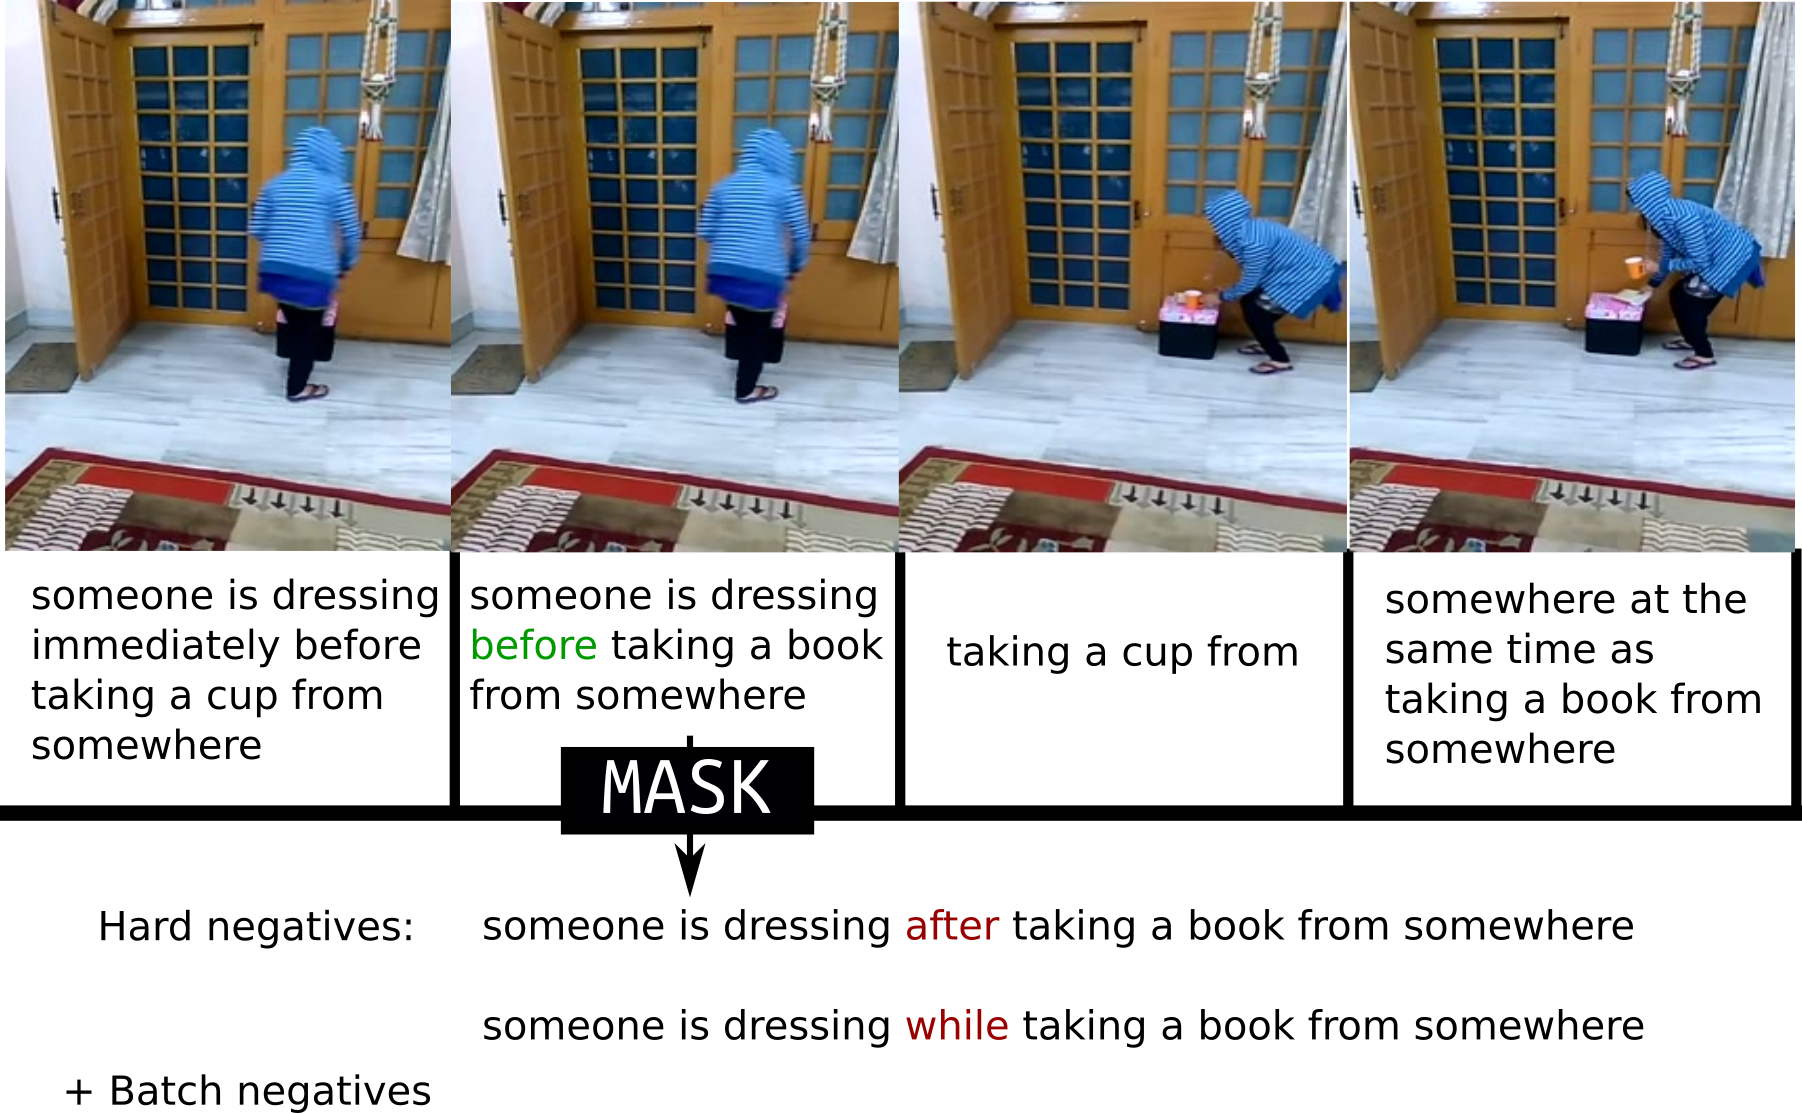
\includegraphics[width=0.8\textwidth]{hard_negatives}
	\caption{Example of annotation with hard negatives for temporal words}
	\label{fig:hard_neg}
\end{figure}
